\documentclass{article}
% Package and macro definitions for CSC 503
% Originally prepared August 23, 2012 by Jon Doyle

%%% Page dimensions
\setlength{\oddsidemargin}{0in}
\setlength{\evensidemargin}{0in}
\setlength{\topmargin}{0in}
\setlength{\textheight}{9in}
\setlength{\textwidth}{6.5in}
\setlength{\headheight}{0in}
\setlength{\headsep}{0in}
\setlength{\footskip}{0.5in}

%%% Font and symbol definition packages
\usepackage{times} 
\usepackage{helvet} 
\usepackage{alltt}
\usepackage{amsfonts, amsmath}
\usepackage{amssymb}

%%% The modified Sellinger fitch.sty file
\input{fitchhr.sty}

\newcommand{\Z}{\mathbb{Z}}
\newcommand{\Q}{\mathbb{Q}}
\newcommand{\R}{\mathbb{R}}
\newcommand{\N}{\mathbb{N}}
\def\land{\wedge}
\def\lor{\vee}
\def\implies{\rightarrow}
\def\iff{\leftrightarrow}
\def\turn{\vdash}
\def\Cn{\text{Cn}}
\def\Th{\text{Th}}
\def\defeq{\stackrel{\rm def}{=}}

%%% The environment for providing answers to problems
\newenvironment{answer}%
{\par\noindent\textbf{Answer}\par\noindent}%
{}


\usepackage{amsfonts, amsmath, amsthm}
\usepackage{tikz}
\usetikzlibrary{arrows,automata}

\def\Sometime{\mathord{\mathsf{F}}}
\def\Forever{\mathord{\mathsf{G}}}
\def\Next{\mathord{\mathsf{O}}}
\def\NextX{\mathord{\mathsf{X}}}
\def\Until{\mathrel{\mathsf{U}}}
\def\Release{\mathrel{\mathsf{R}}}
\def\WeakUntil{\mathrel{\mathsf{W}}}
\def\Before{\mathrel{\mathsf{B}}}
\def\True{\mathord{\mathsf{true}}}
\def\All{\mathord{\mathsf{A}}}
\def\Exists{\mathord{\mathsf{E}}}
\def\Every{\mathord{\mathsf{E}}}

\title{CSC 503 Homework Assignment 8}
\author{Due October 27, 2014}
\date{October 20, 2014}

\begin{document}
\maketitle

\begin{itemize}
\item \textbf{[80 points total]} Consider the transition model ${\cal M}_1$
  depicted in Figure \ref{f1}.
  \begin{figure}[h]
    \centering
    \caption{Model ${\cal M}_1$}
\begin{center}

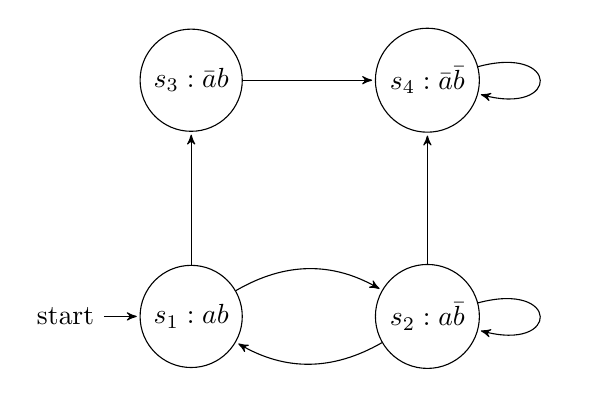
\begin{tikzpicture}[>=stealth',shorten >=1pt,auto,node distance=3cm]
  \node[state] (q3)      {$s_3: \bar a b$};
  \node[state] (q4)    [right of=q3] {$s_4: \bar a \bar b$};
  \node[initial,state] (q1)   [below of=q3]   {$s_1: a b$};
  \node[state] (q2)   [right of=q1]   {$s_2:  a \bar b$};

  \path[->] 
        (q3) edge         node {} (q4)
        (q4) edge [loop right] node {} (q4)
        (q1) edge         node {} (q3)
        (q2) edge         node {} (q4)
        (q2) edge [loop right] node {} (q2)
        (q1) edge    [bend left] node {} (q2)
        (q2) edge    [bend left] node {} (q1);
\end{tikzpicture}
\end{center}
\label{f1}
\end{figure}
  \par
  In answering the following questions, recall that all paths are
  infinite.  To indicate a path that ends with a repeated set of
  states, put parenthesis around the repeated subsequence (e.g., $(q,
  q'', q''')$.  To indicate a path in which an initial subsequence is
  followed by any possible continuing path, write ``(any)'' after
  giving the initial sequence.
  \begin{enumerate}
  \item \textbf{[8 points]} Find a path from the initial state $s_1$
    which satisfies $\Forever a$.
  \item \textbf{[8 points]} Determine whether ${\cal M}_1, s_1 \models
    \Forever a$ and explain why or why not.
  \item \textbf{[8 points]} Find a path from the initial state $s_1$
    which satisfies $a \Until b$.
  \item \textbf{[8 points]} Determine whether ${\cal M}_1, s_1 \models
    a \Until b$ and explain why or why not.
  \item \textbf{[8 points]} Find a path from the initial state $s_1$
    which satisfies $\NextX a \Until \NextX (\neg a \land b)$.
  \item \textbf{[8 points]} Determine whether ${\cal M}_1, s_1 \models
    \NextX a \Until \NextX (\neg a \land b)$ and explain why or why not.
  \item \textbf{[8 points]} Find a path from the initial state $s_1$
    which satisfies $\NextX \neg b \land \Forever (a \lor \neg b)$.
  \item \textbf{[8 points]} Determine whether ${\cal M}_1, s_1 \models
    \NextX \neg b \land \Forever (a \lor \neg b)$ and explain why or why not.
  \item \textbf{[8 points]} Find a path from the initial state $s_1$
    which satisfies $\NextX (\neg a \land b) \land \Sometime (\neg a
    \land \neg b)$.
  \item \textbf{[8 points]} Determine whether ${\cal M}_1, s_1 \models
    \NextX (\neg a \land b) \land \Sometime (\neg a \land \neg b)$ and explain why or why not.
  \end{enumerate}

\item \textbf{[20 points]} List all subformulas of the LTL formula
  \begin{displaymath}
    \NextX \neg p \Until (q \Until ((\Forever r \lor \NextX \Sometime
    \neg q) \implies \NextX r \WeakUntil \neg q))
  \end{displaymath}
\end{itemize}

\end{document}
